%% 
%% Copyright 2007-2020 Elsevier Ltd
%% 
%% This file is part of the 'Elsarticle Bundle'.
%% ---------------------------------------------
%% 
%% It may be distributed under the conditions of the LaTeX Project Public
%% License, either version 1.2 of this license or (at your option) any
%% later version.  The latest version of this license is in
%%    http://www.latex-project.org/lppl.txt
%% and version 1.2 or later is part of all distributions of LaTeX
%% version 1999/12/01 or later.
%% 
%% The list of all files belonging to the 'Elsarticle Bundle' is
%% given in the file `manifest.txt'.
%% 

%% Template article for Elsevier's document class `elsarticle'
%% with numbered style bibliographic references
%% SP 2008/03/01
%%
%% 
%%
%% $Id: elsarticle-template-num.tex 190 2020-11-23 11:12:32Z rishi $
%%
%%
\documentclass[preprint,12pt]{elsarticle}

%% Use the option review to obtain double line spacing
%% \documentclass[authoryear,preprint,review,12pt]{elsarticle}

%% Use the options 1p,twocolumn; 3p; 3p,twocolumn; 5p; or 5p,twocolumn
%% for a journal layout:
%% \documentclass[final,1p,times]{elsarticle}
%% \documentclass[final,1p,times,twocolumn]{elsarticle}
%% \documentclass[final,3p,times]{elsarticle}
%% \documentclass[final,3p,times,twocolumn]{elsarticle}
%% \documentclass[final,5p,times]{elsarticle}
%% \documentclass[final,5p,times,twocolumn]{elsarticle}

%% For including figures, graphicx.sty has been loaded in
%% elsarticle.cls. If you prefer to use the old commands
%% please give \usepackage{epsfig}

%% The amssymb package provides various useful mathematical symbols
\usepackage{amssymb}
%% The amsthm package provides extended theorem environments
%% \usepackage{amsthm}

%% The lineno packages adds line numbers. Start line numbering with
%% \begin{linenumbers}, end it with \end{linenumbers}. Or switch it on
%% for the whole article with \linenumbers.
%% \usepackage{lineno}

\journal{Lancet Public Health}

\begin{document}

\begin{frontmatter}

%% Title, authors and addresses

%% use the tnoteref command within \title for footnotes;
%% use the tnotetext command for theassociated footnote;
%% use the fnref command within \author or \address for footnotes;
%% use the fntext command for theassociated footnote;
%% use the corref command within \author for corresponding author footnotes;
%% use the cortext command for theassociated footnote;
%% use the ead command for the email address,
%% and the form \ead[url] for the home page:
%% \title{Title\tnoteref{label1}}
%% \tnotetext[label1]{}
%% \author{Name\corref{cor1}\fnref{label2}}
%% \ead{email address}
%% \ead[url]{home page}
%% \fntext[label2]{}
%% \cortext[cor1]{}
%% \affiliation{organization={},
%%             addressline={},
%%             city={},
%%             postcode={},
%%             state={},
%%             country={}}
%% \fntext[label3]{}

\title{Transportation systems and pollution in cities in 2020}

%% use optional labels to link authors explicitly to addresses:
%% \author[label1,label2]{}
%% \affiliation[label1]{organization={},
%%             addressline={},
%%             city={},
%%             postcode={},
%%             state={},
%%             country={}}
%%
%% \affiliation[label2]{organization={},
%%             addressline={},
%%             city={},
%%             postcode={},
%%             state={},
%%             country={}}

\author[melb]{Kerry~A.~Nice\corref{cor1}}
\cortext[cor1]{Principal corresponding author}
\ead{kerry.nice@unimelb.edu.au}
\address[melb]{Transport, Health, and Urban Design Research Lab, Faculty of Architecture, Building, and Planning, University of Melbourne, VIC, Australia.}
%\address[eng]{Melbourne School of Engineering; and Melbourne School of Population and Global Health, University of Melbourne, VIC, Australia.}

%\affiliation{organization={},%Department and Organization
%            addressline={}, 
%            city={},
%            postcode={}, 
%            state={},
%            country={}}

%\begin{abstract}
%% Text of abstract

%\end{abstract}

%%Graphical abstract
%\begin{graphicalabstract}
%\includegraphics{grabs}
%\end{graphicalabstract}

%%Research highlights
%\begin{highlights}
%\item Research highlight 1
%\item Research highlight 2
%\end{highlights}

%\begin{keyword}
%% keywords here, in the form: keyword \sep keyword

%% PACS codes here, in the form: \PACS code \sep code

%% MSC codes here, in the form: \MSC code \sep code
%% or \MSC[2008] code \sep code (2000 is the default)

%\end{keyword}

\end{frontmatter}

%% \linenumbers

%% main text

\section{Summary}
\textbf{Background} This is the background. It is two sentences.

\textbf{Methods} This is a paragraph of methods.

\textbf{Findings} This is a paragraph of findings.

\textbf{Interpretation} This is the interpretation. It is three sentences.

\textbf{Funding} States the funding sources.

\section{Research in context}

\textbf{Evidence before this study} 
A paragraph about what existed before.

\textbf{Added value of this study} 
A paragraph about what the study provides.

\textbf{Implications of all the available evidence} 
A paragraph about the implications of the study.

\section{Introduction}
This has a short introduction, three paragraphs or so.

\section{Methods}

\subsection{Data sources}


\begin{figure}
\centering
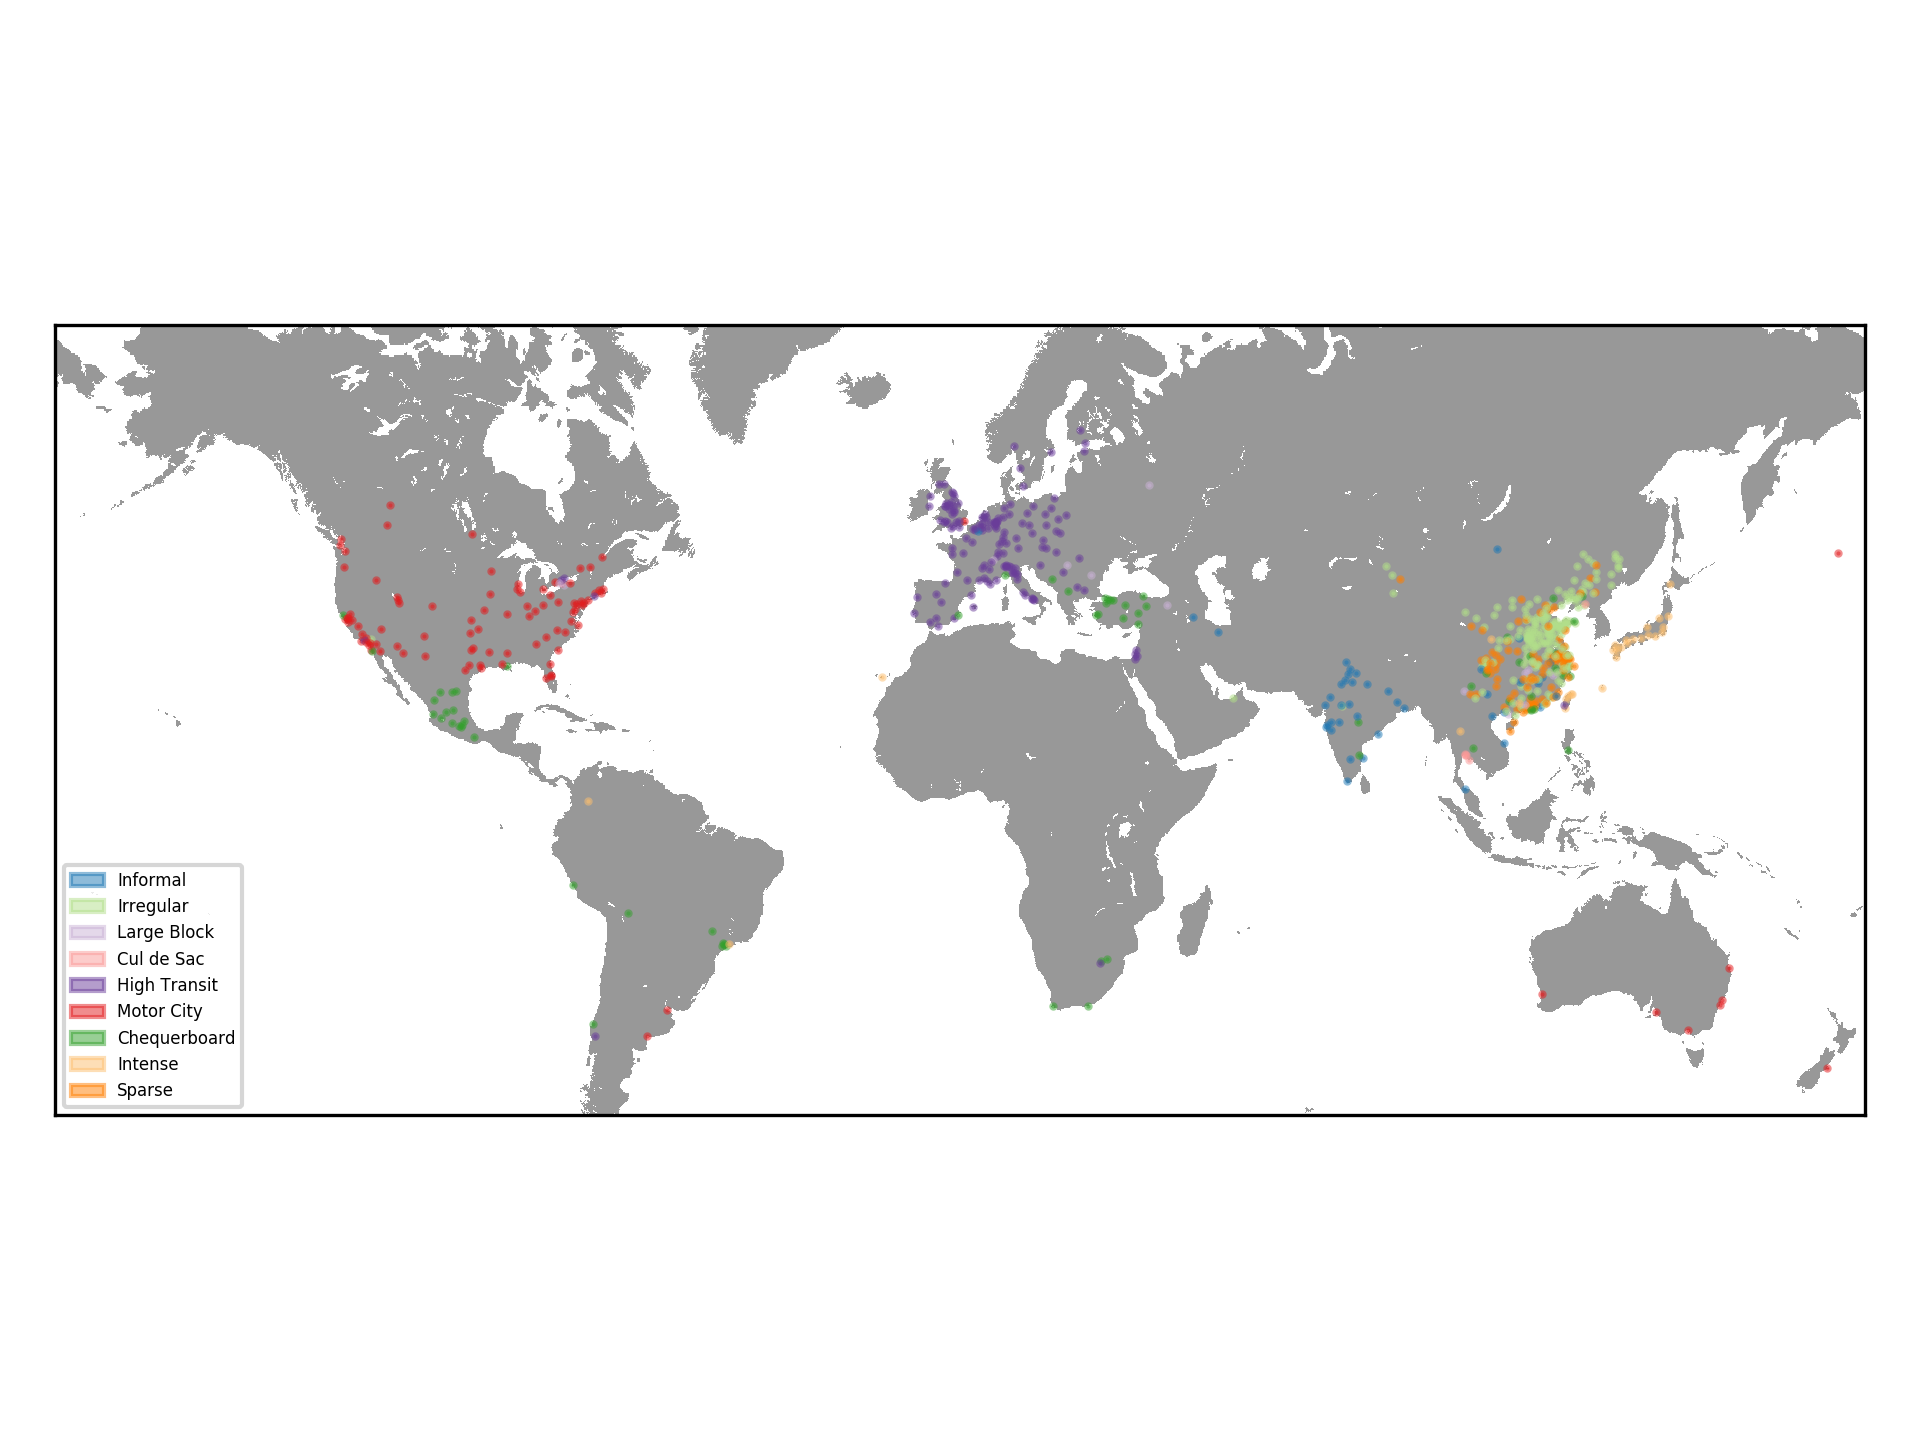
\includegraphics[trim={13 78 13 78},clip,scale=0.9]{Images/WorldPollutionClusters.png}
\caption{\bf Locations and urban typologies of the 679 cities used in this study.}
 \label{fig:clusters}
\end{figure}

Nine global city types were derived in Thompson et al. (2020) \cite{Thompson2020} through visual classification techniques clustering similarities in urban design and transportation networks. These types were defined as high transit (HTR), motor cities (MOT), intense (INT), cul de sac (CUL), Chequerboard (CHQ), informal (INF), irregular (IRR), large block (LBR), sparse (SPR). 

INF cities (n=365) are sparse with low capacity road infrastructure and low amount of formal green space located mostly in Western China and rural India. IRR cities (n=311) have high green space, a mix of formal and high capacity road networks and low mass transit networks and are primary located in Eastern China. LBR cities (n=146) feature medium density formal low and high capacity road networks and medium amount of rail transport and are mostly located in Russia and Eastern Europe. CUL cities (n=26) feature very high density, low capacity mixed formal and informal road networks, with low levels of mass transit and are spread across India, Indonesia, Vietnam, Philippines, and Thailand. HTR cities (n=163) have medium density, high capacity formal road networks with high public transport and are predominately located in Western Europe. MOT cities (n=158) are medium to low density, have high capacity grid based road networks with medium railed transport and are prevalent in North America and Australia. CHQ cities (n=257) are high density, medium capacity mixed formal and informal road networks with medium public transportation and consist of Spanish and Portuguese cities and their colonial cities in Latin America. INT cities (n=22) are very high density, mixed formal high capacity and informal road networks with high public tranport and are mostly Japanese, Columbian, and high density Asian island cities such as Singapore. SPR cities feature low capacity, low density formal and informal road networks with low public transport and are mostly in Western China.



Wijnands et al. (2022) \cite{Wijnands2022} created pollutant and city specific XGBoost models for 679 cities, trained on weather and pollution observations over 2015-2019 and used these models to predict daily pollution levels of NO$_{2}$, PM$_{2.5}$, PM$_{10}$, and O$_{3}$ over 2020. Using 2020 observed values, anomalies were calculated in the absence of a pandemic. The original Thompson et al. (2020) urban typology dataset consisted of the largest 1632 cities in the world. Of these, a subset of 679 cities were used (see Figure \ref{fig:clusters}), those that had pollution data available.








\subsection{Data analysis}
The methods part 2.


\section{Results}
Maybe a page of text and some graphs.


\begin{figure}
\centering
\includegraphics[trim={0 19 22 43},clip,scale=0.45]{Images/no2CulmReductionClusterMean_2020.png}
\caption{\bf Cumulative daily mean NO$_{2}$ anomalies over 2020 per urban typology type, calculated as a daily percent difference over a January 1-10th, 2020 baseline and summed daily. }
 \label{fig:no2}
\end{figure}

\begin{figure}
\centering
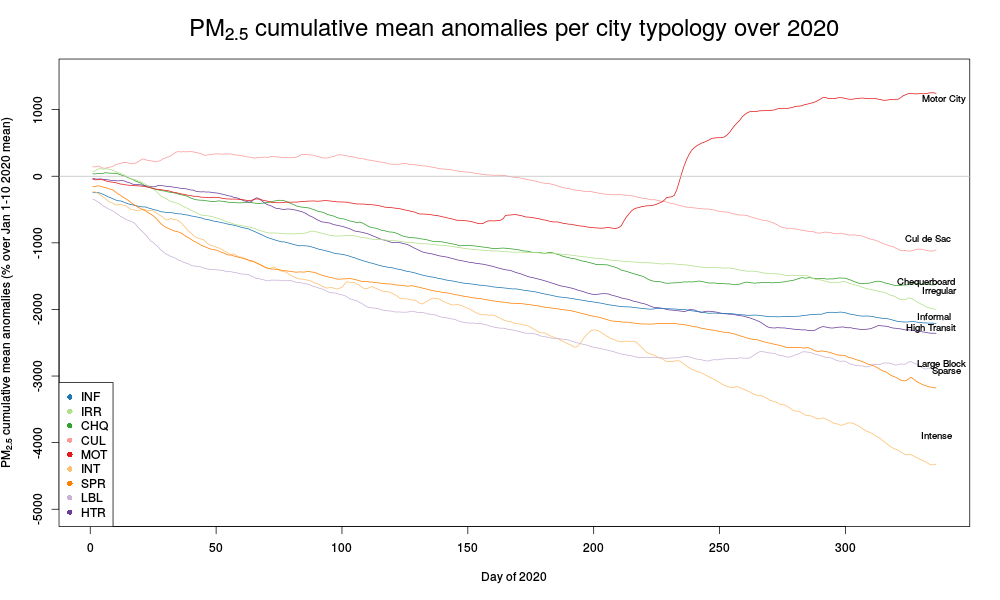
\includegraphics[trim={0 19 22 43},clip,scale=0.45]{Images/pm25CulmReductionClusterMean_2020.png}
\caption{\bf  Cumulative mean PM$_{2.5}$ anomalies over 2020 per urban typology type, calculated as a daily percent difference over a January 1-10th, 2020 baseline and summed daily.}
 \label{fig:pm25}
\end{figure}

\begin{figure}
\centering
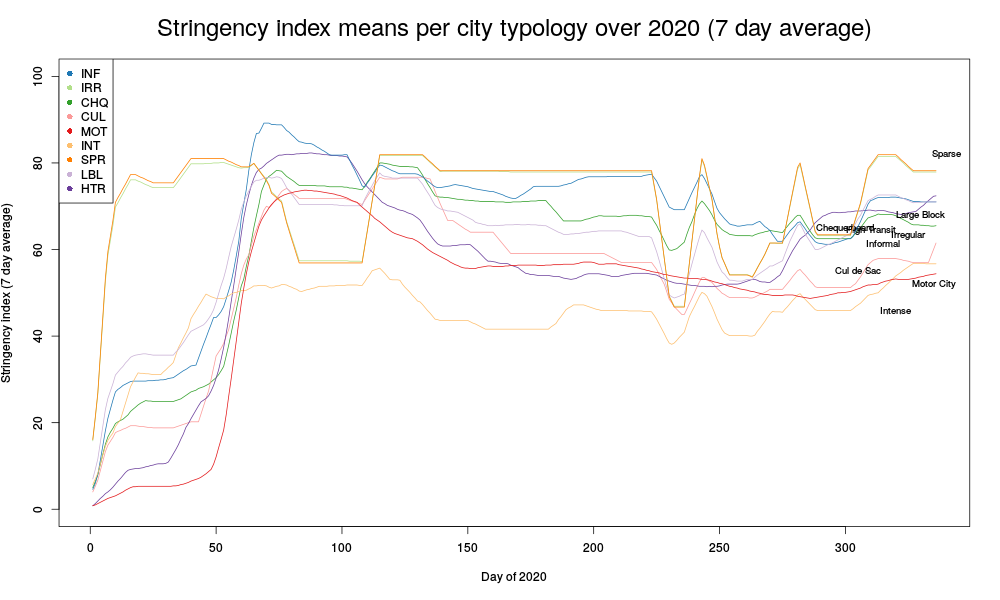
\includegraphics[trim={0 19 22 43},clip,scale=0.25]{Images/LocalStringencyClusterMean7Ave_2020.png}
\caption{\bf  Stringency index (7 day running average) per urban typology type over 2020.}
 \label{fig:string}
\end{figure}

\begin{figure}
\centering
\includegraphics[trim={0 19 22 43},clip,scale=0.25]{Images/Descarte_mobilityClusterMean7Ave_2020.png}
\caption{\bf  Descartes mobility index (7 day running average) per urban typology type over 2020.}
 \label{fig:desc}
\end{figure}



\begin{figure}
\centering
\includegraphics[trim={0 19 22 43},clip,scale=0.25]{Images/CovidCasesClusterMean7Ave_2020.png}
\caption{\bf  COVID-19 cases per 100,000 (7 day running average) per urban typology type over 2020.}
 \label{fig:covidcases}
\end{figure}




\begin{figure}
{\tiny a)}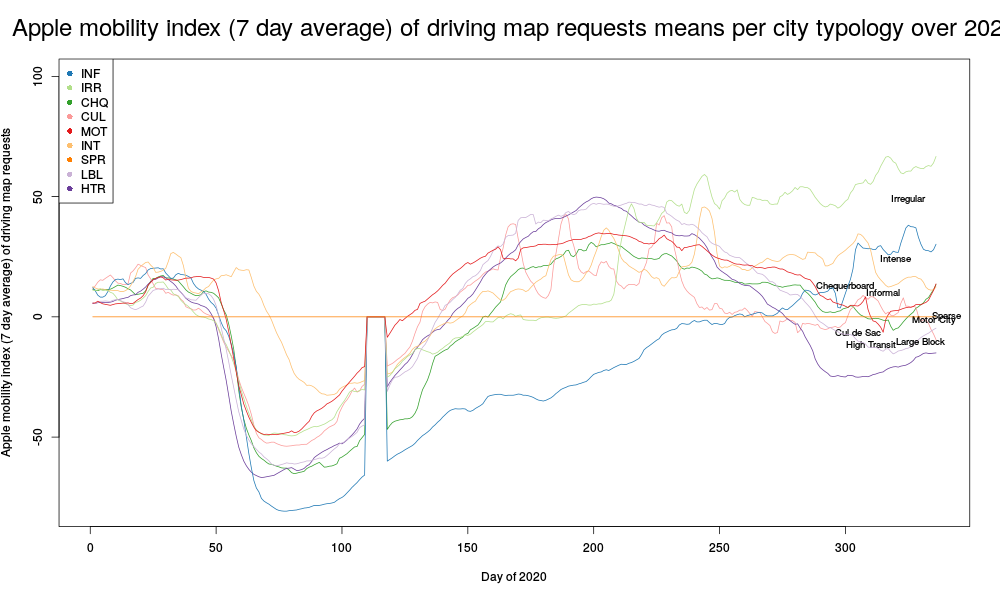
\includegraphics[trim={0 19 22 43},clip,scale=0.23]{Images/AppleDrivingClusterMean7Ave_2020.png}~
{\tiny b)}\includegraphics[trim={0 19 22 43},clip,scale=0.23]{Images/AppleTransitClusterMean_20207Ave.png}
\\
{\tiny c)}\includegraphics[trim={0 19 22 43},clip,scale=0.23]{Images/GoogleTransitClusterMean7Ave_2020.png}~
{\tiny d)}\includegraphics[trim={0 19 22 43},clip,scale=0.23]{Images/GoogleWorkplacesClusterMean7Ave_2020.png}
\caption{\bf a) Apple mobility index (7 day running average) of map requests for driving directions per urban typology type over 2020. b) Apple mobility index (7 day running average) of map requests for transit directions per urban typology type over 2020. c) Google mobility index (7 day running average) of transit locations per urban typology type over 2020. d) Google mobility index (7 day running average) of workplace locations per urban typology type over 2020.}
 \label{fig:driving}
\end{figure}



%\begin{figure}
%\centering
%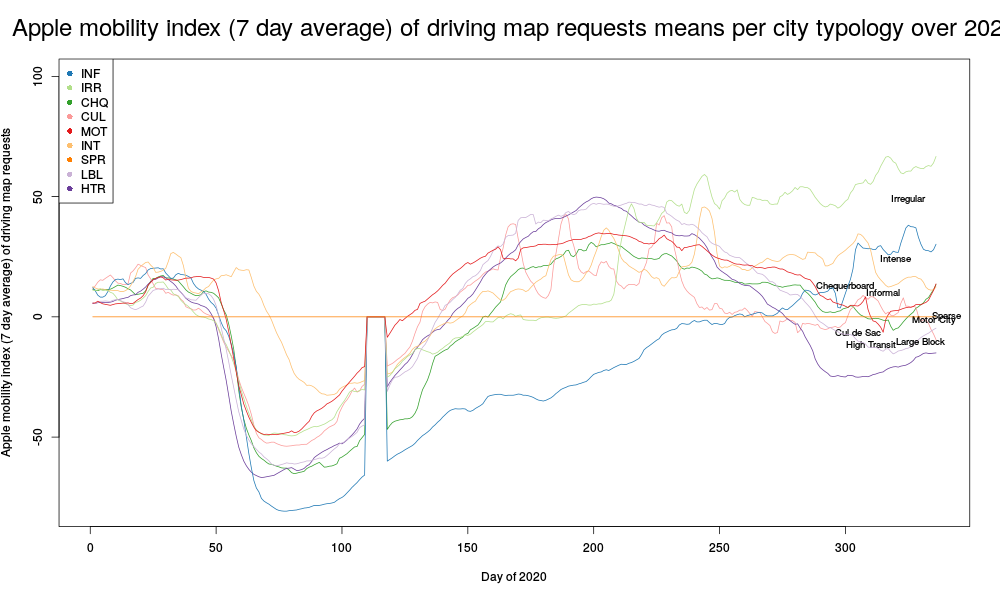
\includegraphics[trim={0 19 22 43},clip,scale=0.25]{Images/AppleDrivingClusterMean7Ave_2020.png}
%\caption{\bf Apple mobility index (7 day running average) of map requests for driving directions per urban typology type over 2020.}
% \label{fig:driving}
%\end{figure}
%
%\begin{figure}
%\centering
%\includegraphics[trim={0 19 22 43},clip,scale=0.25]{Images/AppleTransitClusterMean_20207Ave.png}
%\caption{\bf Apple mobility index (7 day running average) of map requests for transit directions per urban typology type over 2020.}
% \label{fig:transit}
%\end{figure}
%
%\begin{figure}
%\centering
%\includegraphics[trim={0 19 22 43},clip,scale=0.25]{Images/GoogleTransitClusterMean7Ave_2020.png}
%\caption{\bf Google mobility index (7 day running average) of transit locations per urban typology type over 2020.}
% \label{fig:gtransit}
%\end{figure}
%
%\begin{figure}
%\centering
%\includegraphics[trim={0 19 22 43},clip,scale=0.25]{Images/GoogleWorkplacesClusterMean7Ave_2020.png}
%\caption{\bf Google mobility index (7 day running average) of workplace locations per urban typology type over 2020.}
% \label{fig:gwork}
%\end{figure}





\section{Discussion}
A page or two of discussion (that also includes the conclusion).

\section{Contributors}\label{sec:credit}
\textbf{KAN}: Conceptualization, Methodology, Software, Formal Analysis, Writing - Original Draft, Writing - Review \& Editing, Visualization.

\section{Declaration of interests}\label{sec:dec}
We declare no competing interests.

\section{Acknowledgments}\label{sec:ak}
KAN is supported by NHMRC/UKRI grant (1194959).


%\section{}
%\label{}

%% The Appendices part is started with the command \appendix;
%% appendix sections are then done as normal sections
%% \appendix

%% \section{}
%% \label{}

%% If you have bibdatabase file and want bibtex to generate the
%% bibitems, please use
%%
%%  \bibliographystyle{elsarticle-num} 
%%  \bibliography{<your bibdatabase>}

%% else use the following coding to input the bibitems directly in the
%% TeX file.

\section{References}\label{sec:ref}
\begin{thebibliography}{00}

%% \bibitem{label}
%% Text of bibliographic item

%\bibitem{}
\bibliographystyle{elsarticle-num} 
\bibliography{bib}


\end{thebibliography}
\end{document}
\endinput
%%
%% End of file `elsarticle-template-num.tex'.
